% Options for packages loaded elsewhere
\PassOptionsToPackage{unicode}{hyperref}
\PassOptionsToPackage{hyphens}{url}
%
\documentclass[
  11pt,
]{article}
\usepackage{lmodern}
\usepackage{amssymb,amsmath}
\usepackage{ifxetex,ifluatex}
\ifnum 0\ifxetex 1\fi\ifluatex 1\fi=0 % if pdftex
  \usepackage[T1]{fontenc}
  \usepackage[utf8]{inputenc}
  \usepackage{textcomp} % provide euro and other symbols
\else % if luatex or xetex
  \usepackage{unicode-math}
  \defaultfontfeatures{Scale=MatchLowercase}
  \defaultfontfeatures[\rmfamily]{Ligatures=TeX,Scale=1}
\fi
% Use upquote if available, for straight quotes in verbatim environments
\IfFileExists{upquote.sty}{\usepackage{upquote}}{}
\IfFileExists{microtype.sty}{% use microtype if available
  \usepackage[]{microtype}
  \UseMicrotypeSet[protrusion]{basicmath} % disable protrusion for tt fonts
}{}
\makeatletter
\@ifundefined{KOMAClassName}{% if non-KOMA class
  \IfFileExists{parskip.sty}{%
    \usepackage{parskip}
  }{% else
    \setlength{\parindent}{0pt}
    \setlength{\parskip}{6pt plus 2pt minus 1pt}}
}{% if KOMA class
  \KOMAoptions{parskip=half}}
\makeatother
\usepackage{xcolor}
\IfFileExists{xurl.sty}{\usepackage{xurl}}{} % add URL line breaks if available
\IfFileExists{bookmark.sty}{\usepackage{bookmark}}{\usepackage{hyperref}}
\hypersetup{
  pdftitle={Variation in histone configurations correlates with gene expression across nine inbred strains of mice},
  hidelinks,
  pdfcreator={LaTeX via pandoc}}
\urlstyle{same} % disable monospaced font for URLs
\usepackage[margin=1in]{geometry}
\usepackage{graphicx}
\makeatletter
\def\maxwidth{\ifdim\Gin@nat@width>\linewidth\linewidth\else\Gin@nat@width\fi}
\def\maxheight{\ifdim\Gin@nat@height>\textheight\textheight\else\Gin@nat@height\fi}
\makeatother
% Scale images if necessary, so that they will not overflow the page
% margins by default, and it is still possible to overwrite the defaults
% using explicit options in \includegraphics[width, height, ...]{}
\setkeys{Gin}{width=\maxwidth,height=\maxheight,keepaspectratio}
% Set default figure placement to htbp
\makeatletter
\def\fps@figure{htbp}
\makeatother
\setlength{\emergencystretch}{3em} % prevent overfull lines
\providecommand{\tightlist}{%
  \setlength{\itemsep}{0pt}\setlength{\parskip}{0pt}}
\setcounter{secnumdepth}{-\maxdimen} % remove section numbering

\newcommand{\beginsupplement}{%
        \setcounter{table}{0}
        \renewcommand{\thetable}{S\arabic{table}}%
        \setcounter{figure}{0}
        \renewcommand{\thefigure}{S\arabic{figure}}%
     }

\usepackage{natbib}

\usepackage{setspace} \doublespacing

\usepackage{fancyhdr}
\pagestyle{fancy}
\lhead{Tyler, Spruce, et al.}
\rhead{Epigenetic variation in nine inbred mouse strains}

\bibliographystyle{genome_research}
\ifluatex
  \usepackage{selnolig}  % disable illegal ligatures
\fi

\title{Variation in histone configurations correlates with gene
expression across nine inbred strains of mice}
\author{}
\date{\vspace{-2.5em}}

\begin{document}
\maketitle

Anna L. Tyler\textsuperscript{1,$*$}, Catrina
Spruce\textsuperscript{1,$*$}, Romy Kursawe\textsuperscript{2}, Annat
Haber\textsuperscript{2}, Robyn L. Ball\textsuperscript{1}, Wendy A.
Pitman\textsuperscript{1}, Alexander D. Fine\textsuperscript{1},
Narayanan Raghupathy\textsuperscript{1}, Michael
Walker\textsuperscript{1}, Vivek M. Philip\textsuperscript{1},
Christopher L. Baker\textsuperscript{1}, J. Matthew
Mahoney\textsuperscript{1}, Gary A. Churchill\textsuperscript{1},
Jennifer J. Trowbridge\textsuperscript{1}, Michael L.
Stitzel\textsuperscript{2}, Kenneth Paigen\textsuperscript{1}, Petko M.
Petkov\textsuperscript{1,$\dagger$}, Gregory W.
Carter\textsuperscript{1,$\dagger$}

\textsuperscript{1} The Jackson Laboratory for Mammalian Genetics, 600
Main St.~Bar Harbor, ME, 04609

\textsuperscript{2}The Jackson Laboratory for Genomic Medicine 299
Farmington Ave, Farmington, CT 06032

\(^*\) equal contribution \(^\dagger\) corresponding authors

Running title: Epigenetic variation in nine inbred mouse strains

\pagebreak

\hypertarget{abstract}{%
\section{Abstract}\label{abstract}}

It is well established that epigenetic features, such as histone
modifications and DNA methylation, are associated with variation in gene
expression across cell types. Less well known is the extent to which
epigenetic states vary across genetically diverse individuals, and
whether such variation corresponds to inter-individual variation in gene
expression. To investigate genetically driven variation in epigenetics,
we conducted a survey of epigenetic modifications and gene expression in
hepatocytes of nine inbred mouse strains. We surveyed four histone
modifications (H3K4me1, H3K4me3, H3K27me3, and H3K27ac), and DNA
methylation. We used ChromHMM to identify 14 chromatin states, each of
which represented a distinct combination of the four histone
modifications. We found that chromatin states varied widely across the
nine strains and that epigenetic state was strongly correlated with
local gene expression. We replicated this correspondence between
chromatin state and gene expression in an independent population of
Diversity Outbred mice in which we imputed local chromatin state. In
contrast, we found that DNA methylation did not vary across the inbred
strains and was not correlated with variation in gene expression in DO
mice. This work suggests that chromatin state is highly influenced by
local genotype and may be a primary mode through which expression
quantitative trait loci (eQTLs) are mediated. Through examples, we
demonstrate that naturally occurring chromatin state variation, in
conjunction with gene expression, can aid in functional annotation of
the mouse genome. Finally, we provide a data resource that documents
variation in chromatin state in hepatocytes across genetically distinct
mice.

\hypertarget{introduction}{%
\section{Introduction}\label{introduction}}

Although different cell types in an organism house the same genome, each
has a distinct pattern of gene expression. These cell-type specific
patterns of expression are established through epigenetic modification
of both histones \citep{pmid32671792, pmid29625185} and DNA methylation
\citep{pmid21701563, pmid20720541}, which influence the accessibility of
DNA to transcription machinery
\citep{lawrence2016lateral, jones2012functions, moore2013dna}.

This variation in epigenetic landscapes across cell types has been
extensively documented \citep{pmid21441907, pmid25693563} and has been
used to richly annotate functional elements in both mouse
\citep{stamatoyannopoulos2012encyclopedia, baker2019tissue, yue2014comparative}
and human genomes \citep{pmid25693563, pmid23595227, pmid20657582}. Such
functional annotations provide insight into mechanisms of gene
regulation. Because the majority of disease-associated genetic variants
discovered in humans are in gene regulatory regions, it has been
suggested that it is the regulation of gene expression, rather than
alteration of protein function, that is the primary mechanism through
which genetic variation confers disease risk
\citep{maurano2012systematic, farh2015genetic, pmid21617055, pmid19474294}.
Detailed epigenomic landscapes, therefore, may provide important
mechanistic insight linking genotype to disease risk.

However, although variation in epigenetic modifications across cell
types has been deeply explored, we have relatively little knowledge of
inter-individual variation in epigenetic modifications. Does genetic
variation across individuals influence the epigenetic landscape? To what
extent does this variation result in altered gene expression? The
generation of a more complete picture of inter-individual variation in
epigenetic modifications will increase our understanding of the
mechanisms of gene regulation, provide insights into the mechanisms
establishing cell type-specific epigenetic landscapes, and improve the
functional annotation of the genome as it relates to the regulation of
gene expression and disease risk.

To investigate the effect of genetic variation on epigenetic variation,
we performed a survey of epigenetic variation in hepatocytes across nine
inbred mouse strains. We included the eight founders of the Diversity
Outbred/Collaborative Cross (DO/CC) \citep{Svenson:2012hq} mice, as well
as DBA/2J, which, along with C57BL/6J, is one of the founders of the
widely used BxD recombinant inbred panel of mice
\citep{Ashbrook:2019bd}. We assayed four histone modifications: H3K4me3,
which is associated with promoter regions
\citep{heintzman2007distinct, pmid15680324}, H3K4me1, which is
associated with enhancer regions \citep{heintzman2007distinct},
H3K27me3, which is associated with polycomb repression
\citep{bonasio2010molecular}, and H3K27ac, which has been associated
with enhancement of active enhancers and promoters
\citep{creyghton2010histone, heintzman2009histone, rada2011unique}. We
also assayed DNA methylation which is associated with repression of
expression \citep{moore2013dna, jones2012functions}.

We used ChromHMM \citep{Ernst:2012ii} to identify 14 chromatin states,
each representing a unique combination of the four histone marks. We
investigated the association between variation in these states and
variation in gene expression across the nine strains. We separately
investigated the relationship between DNA methylation and gene
expression across strains.

We further investigated the relationship between epigenetic state and
gene expression by imputing the 14 chromatin states and DNA methylation
into a population of DO mice. We then mapped gene expression to the
imputed epigenetic states to assess the extent to which eQTLs were
driven by variation in epigenetic modification.

\hypertarget{results}{%
\section{Results}\label{results}}

Both gene expression and epigenetic state were consistent within mouse
strains but varied across the strains suggesting strong genetic
regulation of both modalities. This is seen as a clustering of
individuals from the same strain in principal component plots of
transcriptomic and epigenetic features (Figure \ref{fig:pc_plots}).
Patterns of gene expression (Figure \ref{fig:pc_plots}A), DNA
methylation (Figure \ref{fig:pc_plots}B) and individual histone
modifications (Figure \ref{fig:pc_plots}C-F) clustered in similar
patterns although a relatively small percent of the variation in the
methylome was related to strain. The three subspecies \textit{musculus}
(in red), \textit{castaneous} (in green) and \textit{domesticus} (all
others) were widely separated suggesting that subspecies structure made
up the majority of the observed variance. The \text{domesticus} strains
largely clustered together. These data provide evidence that epigenetic
features relate to gene expression in a manner that is consistent with
the subspecific origin of the mouse strains.

\begin{figure}[ht!]
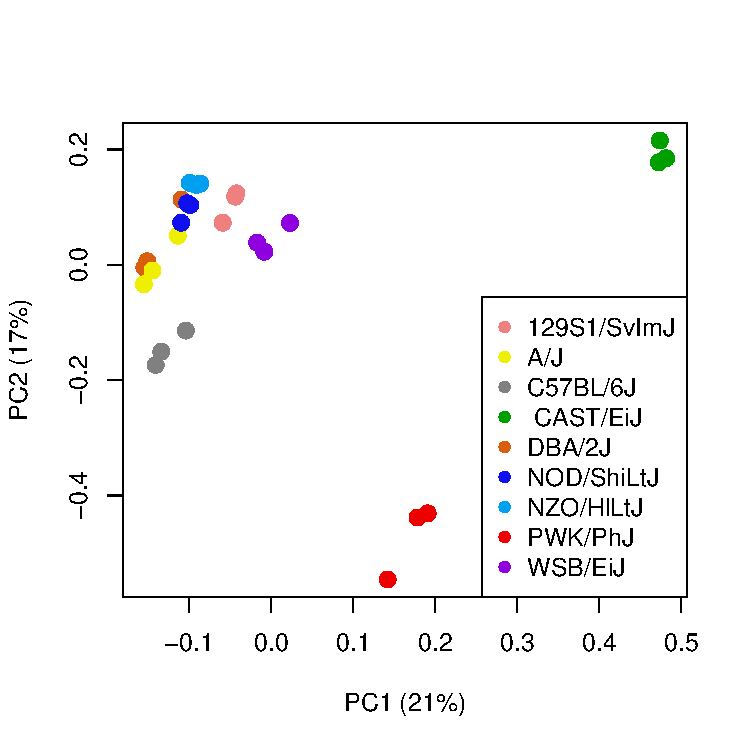
\includegraphics[width=3in]{Figures/Fig1_Decomposition.png} 
\caption{The first two principle components of each genomic 
feature across nine inbred strains of mouse. In all panels 
each point represents an individual mouse, and strain is 
indicated by color as shown in the legend at the bottom of 
the figure. Each panel is labeled with the data used to 
generate the PC plot. (A) Hepatocyte transcriptome - all 
transcripts sequenced in isolated hepatocytes. (B) DNA 
methylation - the percent methylation at all CpG sites 
shared across all individuals. (C-F) Histone modifications - 
the peak heights of the indicated histone modification for 
sites shared across all individuals.}
\label{fig:pc_plots}
\end{figure}

\hypertarget{chromatin-state-overview}{%
\subsection{Chromatin state overview}\label{chromatin-state-overview}}

To investigate the association between histone modifications and gene
expression, we used ChromHMM to identify 14 chromatin states composed of
unique combinations of the four histone modifications. Panel A in Figure
\ref{fig:state_overview} shows the representation of each histone
modification across the states.

\begin{figure}[ht!]
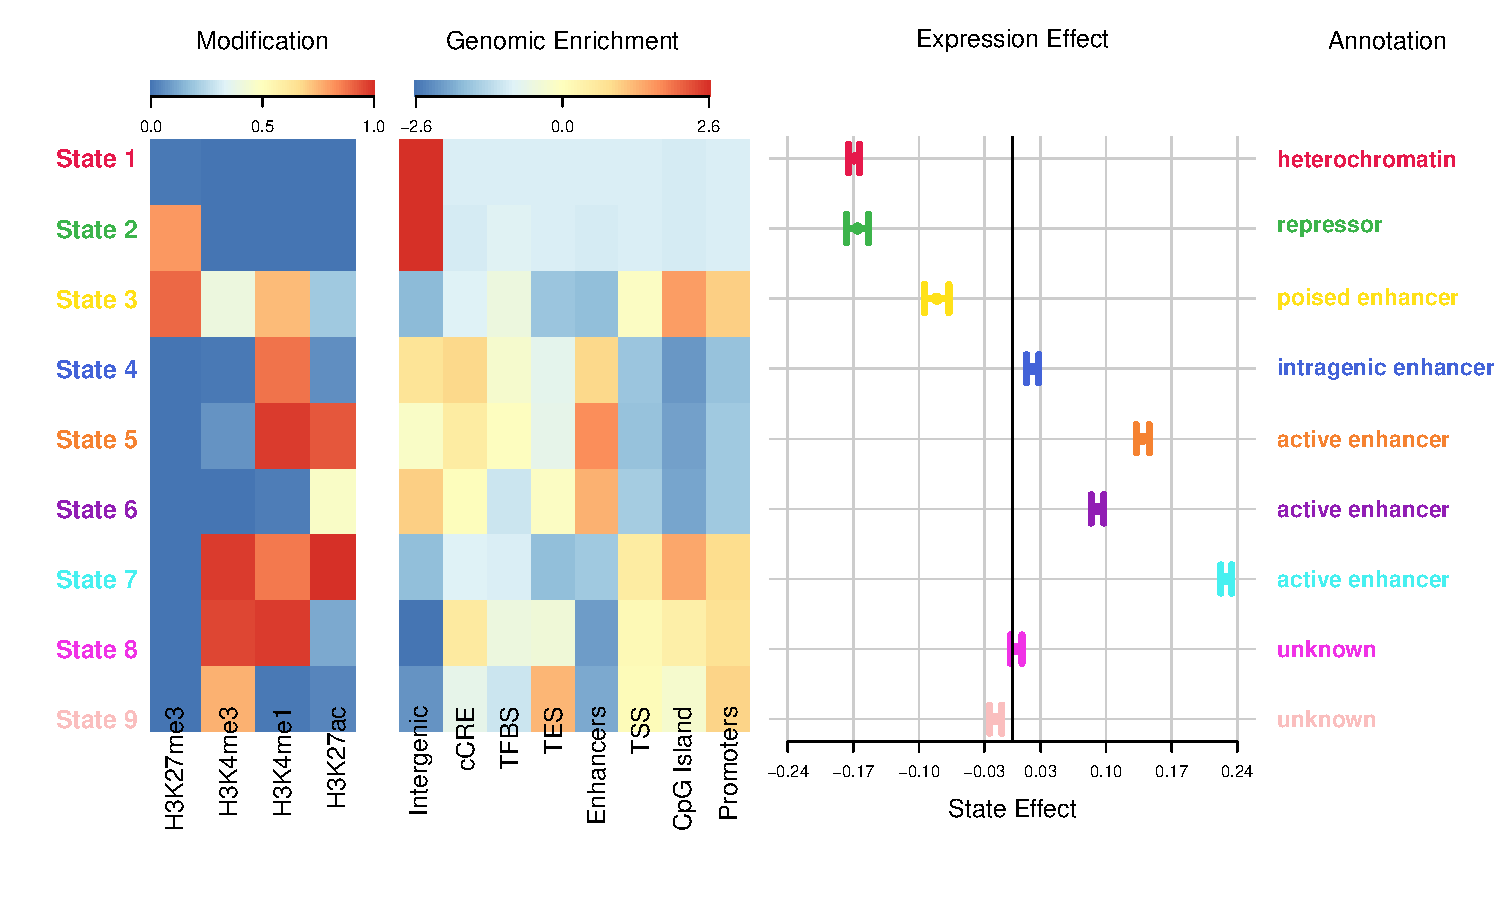
\includegraphics[width=\textwidth]{Figures/Fig2_Overview.png} 
\caption{Overview of chromatin state composition, genomic 
distribution, and effect on expression. (A) Emission 
probabilites for each histone modification in each 
chromatin state. Blue indicates the absence of the histone
modification, and red indicates the presence of the 
modification. (B) The distribution of each state around 
functional elements in the genome. Red indicates that the 
state is enriched near the annotated functional element. 
Blue indicates that the state is depleted near the annotated 
functional element. Abbreviations are as follows: 
TFBS = transcription factor binding sites, cCRE = candidate 
cis-regulatory element, TSS = transcription 
start site, TES = transcription end site. (C) The effect of 
variation in the state on gene expression. Bars are colored 
based on the size and direction the state's effect on expression. 
Darker bars show the effects on expression of chromatin state 
variation across strains. Tan bars show the effects on expression 
of chromatin state variation across genes. (D) Plausible 
annotations for each state based on combining the data in 
the previous three panels. The numbers in parentheses indicate 
the percent of the genome that was assigned to each state.}
\label{fig:state_overview}
\end{figure}

The states were enriched around known functional elements in the mouse
genome (Figure \ref{fig:state_overview}B). For example, the majority of
the states were enriched around transcription start sites (TSS), and
other TSS-related functional elements, such as promoters and CpG
islands. Two states (States 13 and 14) were primarily found in
intergenic regions. Three states (States 2, 6, and 4) were enriched
around known enhancers, and one (State 9) was enriched predominantly
near the transcription end sites (TES).

Most states were also associated with variation in gene expression
across strains (Figure \ref{fig:state_overview}C). The states in Figure
\ref{fig:state_overview} are shown in order of their effect on
expression, which helps illustrate several patterns. The state with the
largest negative effect on gene expression, State 14, is the absence of
all measured modifications. Other states associated with reduced gene
expression contained the repressive mark H3K27me3. The states with the
largest positive effects on expression all had some combination of the
activating marks, H3K4me3, H3K4me1, and H3K27ac. The repressive mark was
less commonly seen in these activating states. These global patterns of
positional enrichment and association with expression largely agree with
previous findings.

By merging the information from Figure \ref{fig:state_overview}A-C, we
were able to suggest annotations for many of the 14 chromatin states
(Figure \ref{fig:state_overview}D). States with the strongest effects on
expression had the clearest annotations, while states with weaker
effects remained unannotated.

\hypertarget{spatial-distribution-of-epigenetic-modifications-around-gene-bodies}{%
\subsection{Spatial distribution of epigenetic modifications around gene
bodies}\label{spatial-distribution-of-epigenetic-modifications-around-gene-bodies}}

In addition to looking for enrichment of chromatin states near annotated
functional elements, we characterized the fine-grained spatial
distribution of each state around gene bodies by normalizing gene
position to run from 0 at the TSS to 1 at the TES (See Methods) (Figure
\ref{fig:state_abundance}A-B). We similarly characterized the
distribution of CpG sites and their percent methylation at this
gene-level scale (Figure \ref{fig:state_abundance}C-D).

\begin{figure}[ht!]
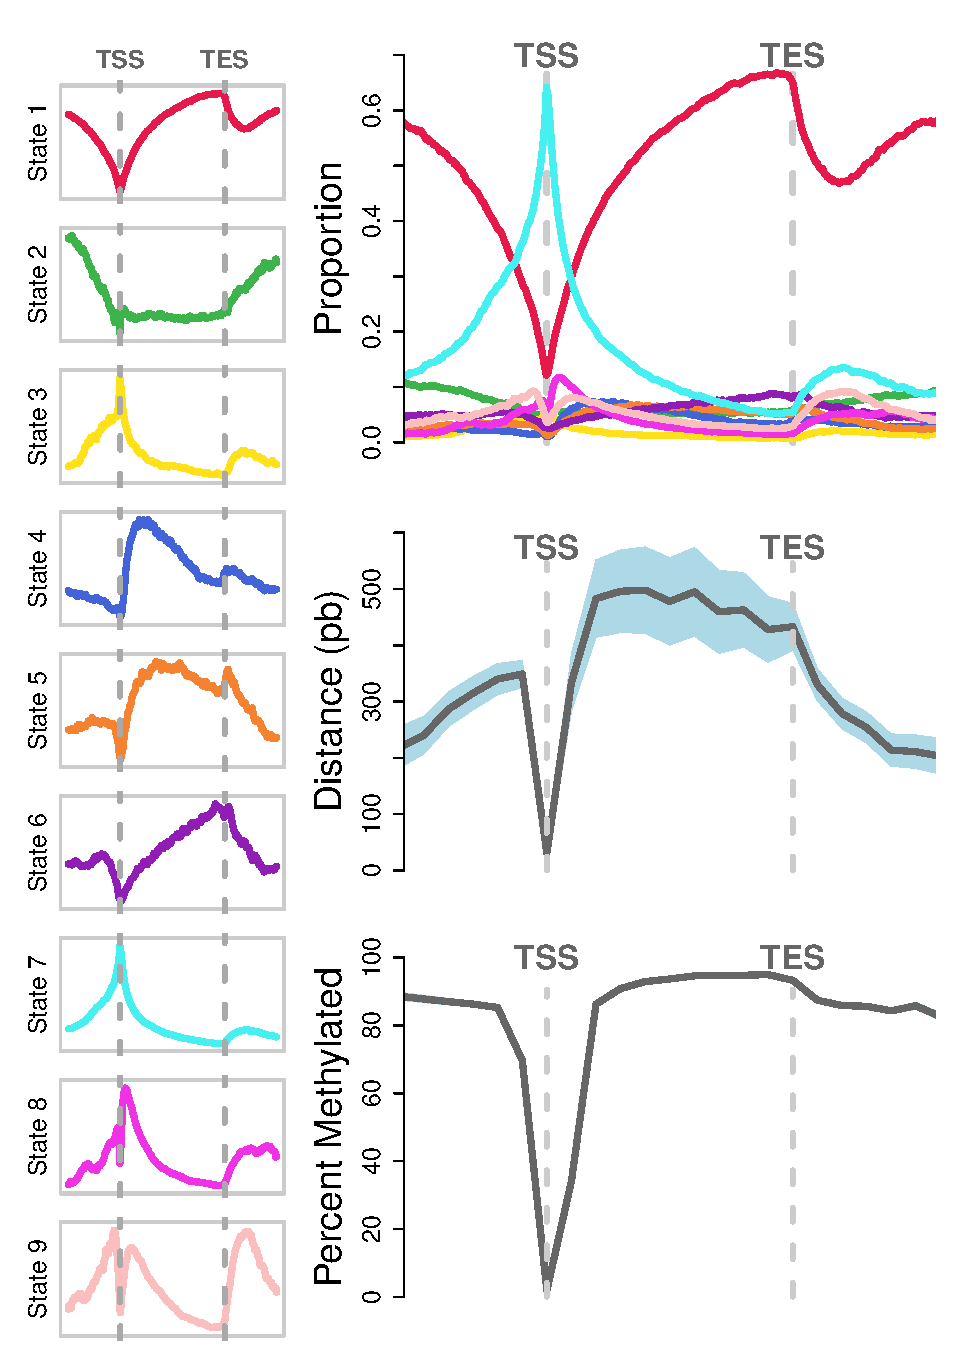
\includegraphics[width=0.67\textwidth]{Figures/Fig3_Abundance.png} 
\caption{Relative abundance of chromatin states and methylated DNA. (A) Each panel 
shows the abundance of a single chromatin state relative to gene TSS and TES. The 
$y$-axis in each panel is the proportion of genes containing the state. Each
panel has an independent $y$-axis to better show the shape of each curve.
The $x$-axis is the relative gene position. The TSS and TES are marked as vertical
gray dashed lines. (B) The same data shown in panel A, but with all states overlayed
onto a single set of axes to show the relative abundance of the states. 
(C) The density of CpG sites relative to the gene body. The $y$-axis shows the 
number of CpG sites per base pair. The density is highest near the TSS. 
CpG sites are less dense within the gene body and in the intergenic space. 
(D) Percent methylation relative to the gene body. The $y$-axis shows the median 
percent methylation at CpG sites, and the $x$-axis shows relative gene position. 
CpG sites near the TSS are unmethylated relative to intragenic and intergenic
CpG sites.}
\label{fig:state_abundance}
\end{figure}

The spatial patterns of the individual chromatin states are shown in
(Figure \ref{fig:state_abundance}A), and an overlay of all states
together (Figure \ref{fig:state_abundance}B) emphasizes the difference
in abundance between the most abundant states (States 1, 3, and 14), and
the remaining states, which were relatively rare.

Each chromatin state had a characteristic distribution pattern. For
example, State 14, which was characterized by the absence of all
measured histone modifications, was strongly depleted near the TSS,
indicating that this region is commonly subject to the histone
modifications we measured here. In contrast, States 1 and 3 were both
enriched at the TSS. State 3 was very narrowly concentrated right at the
TSS, whereas State 1 was more broadly abundant both upstream and
downstream of the TSS. Both were associated overall with increased
expression across inbred mice (indicated by red shading in Figure
\ref{fig:state_abundance}), suggesting promoter or enhancer functions.
The third state in this group of expression-enhancing states, State 2,
was depleted nere the TSS, but enriched within the gene body, suggesting
that this state may mark active intragenic enhancers.

States with weaker effects on expression (indicated by grayer shades in
Figure \ref{fig:state_abundance}) were of lower abundance, but had
distinct distribution patterns around the gene body suggesting the
possibility of distinct functional roles in the regulation of gene
expression.

DNA methylation showed similarly characteristic variation in abundance
(Figure \ref{fig:state_abundance}C-D). The TSS had densely packed CpG
sites relative to the gene body (Figure \ref{fig:state_abundance}C). As
expected, the median CpG site near the TSS was consistently
hypomethylated relative to the median CpG site in intra- and intergenic
regions (Figure \ref{fig:state_abundance}D). All genes used in this
analysis were expressed and thus had some degree of hypomethylation.

\hypertarget{spatially-resolved-effects-on-gene-expression}{%
\subsection{Spatially resolved effects on gene
expression}\label{spatially-resolved-effects-on-gene-expression}}

The distinct spatial distributions of the chromatin states and
methylated CpG sites around the gene body raised the question as to
whether the effects of these states on gene expression could also be
spatially resolved. To investigate this possibility we tested the
association between gene expression and both chromatin state and DNA
methylation using spatially resolved models (Methods). We tested the
effect of each chromatin state on expression across genes within
hepatocytes (Figure \ref{fig:state_effects}A) and the effect of each
chromatin state on the variation in gene expression across strains
(Figure \ref{fig:state_effects}B).

\begin{figure}[ht!]
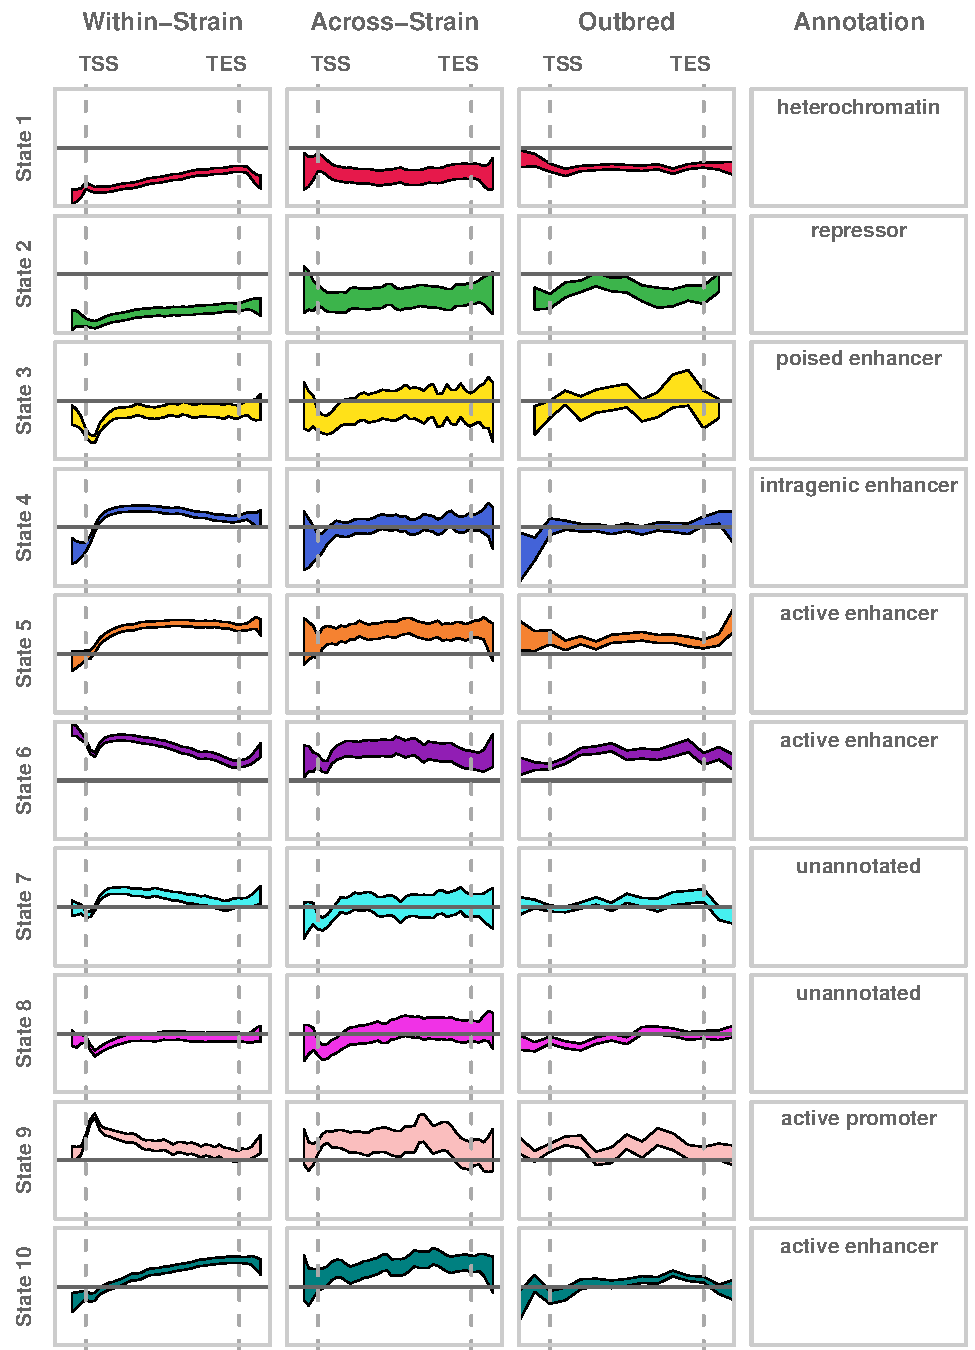
\includegraphics[width=0.7\textwidth]{Figures/Fig4_Effects.png}
\caption{Effects of chromatin states on gene expression. Each column shows 
the effect of the chromatin states on gene expression in a different 
experimental context. The first column shows that the presence of some
states is correlated with higher abundance genes while the presence of
other states is correlated with lower abundance genes in mouse hepatocytes. 
The second column shows that variation in chromatin state across strains
is correlated with variation in gene expression. The third column 
shows the effect of imputed chromatin state on gene expression in a 
population of DO mice. The $y$-axis in each column is constant for comparison
of states to each other within a single context. The $y$-axes vary across
columns to highlight the similarity of the shape of each curve across 
settings. The final column shows the annotation of each state. All $y$-axes 
show the $\beta$ coefficient from the linear model shown in the equation. 
All $x$-axes show the relative position along the gene body. Vertical gray 
dashed lines mark the TSS and TES.}
\label{fig:state_effects}
\end{figure}

All chromatin states demonstrated spatially dependent effects on gene
expression within hepatocytes. For many of the states, the effects on
expression were concentrated at or near the TSS, while in the other
states effects were seen across the whole gene. The direction of the
effects matched the overall effects of each state seen previously
(Figure \ref{fig:state_overview}). The spatial effects were
recapitulated for almost every state when we measured across strains.
That is, chromatin states that either enhanced or suppressed gene
expression across hepatocyte genes were similarly related to variation
in expression across strains. This suggests that the genetic differences
between strains modify chromatin activity in a manner similar to that
used across genes. One notable exception was State 6, whose presence
upregulated genes within hepatocytes, but did not contribute to
expression variation across strains.

We also examined the effect of percent DNA methylation across genes
within hepatocytes and across strains (Figure
\ref{fig:DNA_methylation_effect}). As expected, methylation at the TSS
was associated with lower expression in hepatocytes. However, percent
DNA methylation did not contribute at all to expression variation across
strains. This was in part due to an overall lack of variation in percent
DNA methylation at the TSS. These results imply that percent DNA
methylation does not vary significantly between strains, at least in
hepatocytes, and does not contribute to variation in gene expression
across genetically diverse individuals.

\begin{figure}[ht!]
\includegraphics[width=3in]{Figures/Fig5_methylation_effect.png} 
\caption{Effect of DNA methylation on gene expression (A) across gene expression
in hepatocytes and (B) across inbred strains. The dark gray line shows the
estimate of the effect of percent DNA methylation on gene expression. The 
$x$-axis is normalized position along the gene body running from the 
transcription start site (TSS) to the transcription end site (TES), 
marked with vertical gray dashed lines. The horizontal solid black 
line indicates an effect of 0. The shaded gray area shows 95\% 
confidence interval arond the model fit.}
\label{fig:DNA_methylation_effect}
\end{figure}

\hypertarget{imputed-chromatin-state-explained-expression-variation-in-diversity-outbred-mice}{%
\subsection{Imputed chromatin state explained expression variation in
diversity outbred
mice}\label{imputed-chromatin-state-explained-expression-variation-in-diversity-outbred-mice}}

Thus far, we have used inbred strains of mice to identify correlations
between local chromatin state and gene expression. To compare the
contribution of genetic and epigenetic features to expression
quantitative trait loci (eQTLs) in a gentically diverse population, we
imputed chromatin state, DNA methylation, and SNPs into DO mice
(Methods). Chromatin state is largely determined by local genotype,
especially early in life \citep{pmid16009939}, and can thus be reliably
imputed from local genotype. Further, we have shown here that local
chromatin state correlates with variation in gene expression across
inbred strains. DNA methylation, on the other hand, is known not to be
highly heritable \citep{pmid33931130}, and thus cannot be reliably
imputed from local genotype. We have also shown here that DNA
methylation is not correlated with variation in gene expression across
inbred strains. The imputation of DNA methylation thus serves as a
negative control--an estimate of a lower bound the ability of a feature
imputed from local haplotype to explain gene expression in a new
population.

After imputing each genomic feature into the DO population, we mapped
gene expression to the imputed features and calculated the variance
explained (Methods). The overall distributions of variance explained by
each feature across all transcripts are shown in Figure
\ref{fig:effect_distrubutions}.

\begin{figure}[ht!]
\includegraphics[width=\textwidth]{Figures/Fig6_Imputation.png} 
\caption{Gene expression variance in a DO population explained 
by chromatin state compared to three other genomic features: 
local haplotype, local SNP genotype, and local imputed DNA 
methylation status. A. Distributions of gene expression variance 
explained by each feature. B. Direct comparisons of 
variance explained by local haplotype, and each of the other 
genomic features. Blue lines show $y = x$. Each point is a 
single transcript.}
\label{fig:effect_distrubutions}
\end{figure}

These distributions show the haplotype effect for the marker nearest
each transcript compared with the maximum effect across the gene body
for each of the other imputed features. Overall, local haplotype
explained the largest amount of variance of gene expression in the DO
(\(R^2 = 0.17\); 99\% CI = 0.166-0.174). The variance explained by local
chromatin state was very highly correlated with that of haplotype
(Pearson \(r = 0.96\), 99\% CI = 0.958-0.962) and explained almost as
much variance in gene expression in the DO as local haplotype
(\(R^2 = 0.15\), 99\% CI = 0.143-0.151). The mean variance explained by
SNPs was lower (\(R^2 = 0.13\); 99\% CI = 0.131-0.138) than that
explained by haplotype and was not as highly correlated with local
haplotype as chromatin state was (Pearson \(r = 0.93\); 99\% CI =
0.927-0.933). DNA methylation, the lower bound for variance explained by
a feature imputed from local haplotype, explained the lowest amount of
expression variance in the DO population (\(R^2 = 0.09\); 99\% CI =
0.082-0.088), and had a much lower correlation to haplotype than either
chromatin state or SNPs (Pearson \(r = 0.74\); 99\% CI = 0.728-0.751).
Taken together, these results suggest that the majority of
haplotype-associated variance is encoded by the chromatin state of the
allele. Moreover, this encoding is primarily local and present in the
relevant inbred founder strain.

To investigate whether natural variation in chromatin state can be used
to functionally annotate the mouse genome, we looked at the relationship
between chromatin state and gene expression in individual genes. An
example gene, \textit{Pkd2}, is shown in Figure \ref{fig:example_gene}.
This figure shows chromatin state (Figure \ref{fig:example_gene}B), SNP
genotype (Figure \ref{fig:example_gene}C), and DNA methylation (Figure
\ref{fig:example_gene}D) status along the gene body of \textit{Pkd2}. It
also shows the association of each of these features with gene
expression calculated across the whole gene body (Figure
\ref{fig:example_gene}A).

The detailed view of this gene identifies two particularly interesting
regions. One is at the TSS and the immediately surrounding area, and the
other is just downstream of the TSS.

\begin{figure}[ht!]
\includegraphics[width=0.8\textwidth]{Figures/Fig7_Example.png} 
\caption{Example of epigenetic states and imuptation results for a single 
gene, \textit{Pkd2}. The legend for each panel is displayed to its right.
(A) The variance in DO gene expression explained at 
each position along the gene body by each of the imputed genomic 
features: SNPs - red X's, Chromatin State - blue plus signs, and 
Percent Methylation - green circles. The horizontal dashed line shows 
the variance explained by the haplotype. For reference, the arrow 
below this panel runs from the TSS of \textit{Pkd2} to the TES and 
shows the direction of transcription. (B) The chromatin states assigned 
to each 200 bp window in this gene for each inbred mouse strain. States 
are colored by their effect on gene expression in the inbred mice. Red 
indicates a positive effect on gene expression, and blue indicates a 
negative effect. Each row shows the chromatin states for a single inbred 
strain, which is indicated by the label on the left. (C) SNPs along the 
gene body for each inbred strain. The reference genotype is shown in gray. 
SNPs are colored by genotype as shown in the legend. (D) Percent DNA 
methylation for each inbred strain along the \textit{Pkd2} gene body. 
Percentages are binned into 0\% (blue) 50\% (yellow) and 100\% (red). 
(E) Haplotype effects for expression of \textit{Pkd2} in the DO. 
Haplotype effects are colored by from which each allele was derived. 
(F) \textit{Pkd2} expression levels across inbred mouse strains. For 
ease of comparison, all panels B through F are shown in the same order 
as the haplotype effects.}
\label{fig:example_gene}
\end{figure}

These two regions were both strongly associated expression levels
(Figure \ref{fig:example_gene}A). Those strains with activating histone
states in these regions had much higher expression of \textit{Pkd2} than
the two strains that did not have activating states in this region. We
hypothesize that these two regions are enhancers.

The spatial patterns in the SNPs only partially mirror those in
chromatin state (Figure Figure \ref{fig:example_gene}C). SNPs underlying
the putative enhancer region at the TSS could potentially influence gene
expression by altering local chromatin state. However, the more
downstream enhancer has no underlying SNPs, suggesting that there is an
alternative mechanism for determining chromatin state at this location.
Perhaps SNPs in the TSS region regulate both enhancers.

Percent DNA methylation does not vary across the strains in either of
these putative enhancer regions, and does not contribute to variation in
expression across genetically distinct individuals (Figure
\ref{fig:example_gene}D).

\hypertarget{discussion}{%
\section{Discussion}\label{discussion}}

In this study we showed that genetic variation across inbred mice alters
histone modification patterns in hepatocytes. We further showed that the
variation in histone patterns was highly related to variation in gene
expression across strains. These observations suggest that within a cell
type specific patterns of histone modifications are determined by local
genotype, and are likely a major mechanism through which eQTL are
generated. This hypothesis was supported by the high concordance between
chromatin state, which was imputed from local genotype, and gene
expression in an independent outbred population of mice. Thus, across
cell types, there is likely a strong interaction between factors
determining cell fate, such as transcription factor expression, and
local genetics.

In contrast to chromatin state, percent DNA methylation was not
associated with variation in gene expression across inbred strains or in
the outbred population. At the TSS, this was largely due to a lack of
variation in methylation across strains. An example of this observation
is shown in panel D of Figure \ref{fig:example_gene}. Despite strain
variation in both genotype and chromatin state at the TSS of
\textit{Pkd2}, DNA methylation was invariant -- the CpG island at the
TSS is unmethylated in all strains. Thus, although chromatin state
appears to be highly influenced by local haplotype, percent DNA
methylation is not. CpG islands are highly conserved across vertebrates
\citep{papin2021cpg} and may thus be regions of low genetic variation
within this study relative to the surrounding regions in which SNPs and
variations in histone modifications are abundant.

Variation in DNA methylation has shown a similar lack of association
with gene expression in humans \citep{pmid33931130}. Multiple twin
studies have estimated the average heritability of individual CpG sites
to be roughly 0.19 \citep{pmid27051996, pmid24183450, pmid22532803},
with only about 10\% of CpG sites having a heritability greater than 0.5
\citep{pmid24183450, pmid22532803, pmid24887635}. Trimodal CpG sites,
i.e.~those with methylation percent varying among 0, 50, and 100\%, have
been shown in human brain tissue to be more heritable than unimodal, or
bimodal sites (\(h^2 = 0.8 \pm 0.18\)), and roughly half were associated
with local eQTL \citep{pmid20485568}. Here, we did not see an
association between trimodal CpG sites and gene expression across
strains (Supplemental Figure \ref{supp_fig:trimodal}).

The diversity in the effects observed in the 14 chromatin states
highlights the importance of analyzing combinatorial states as opposed
to individual histone modifications. To illustrate this point, consider
the three states with the largest positive effects on transcription.
Each of these three states had a distinct combination of the three
activatin histone marks: H3K4me1, H3K4me3, and H3K27ac. And although all
three states were associated with increased gene expression, each had a
distinct spatial distribution. This variation in spatial distribution
was mirrored in the spatial effects on transcription. These distinct
patterns would not be detectable without analysis of the histone
modifications in combination. These results highlight the complexity of
the histone code and the importance at analyzing combinatorial states.

While we were able to annotate several states, particularly those with
the strongest effects on gene expression, other states were more
difficult to annotate. This raises the intruiguing possibility of
identifying new modes of expression regulation through histone
modification. One of these unannotated states, State 9, had a weak, but
consistent negative effect on gene transcription centered within the
gene body downstream of the TSS. This state was characterized by high
levels of H3K4me3 and low levels of the other three modifications.

The modification H3K4me3 is most frequently associated with increased
transcriptional activity
\citep{pmid15680324, pmid14661024, pmid12353038, pmid16728976}, so the
association with state 9 with reduced transcription is a deviation from
the dominant paradigm. The physical distribution of this state is also
interesting. It was depleted at the TSS, but enriched just upstream and
just downstream of the TSS. It was also enriched just downstream of the
TES, although it did not appear to influence transcription at this
location. The group of genes marked by State 9 were enriched for
functions such as stress response, DNA damage repair, and ncRNA
processing suggesting that this state may be used to regulate subsets of
genes involved in responses to environmental stimuli.

We detected two bivalent states in this survey. Bivalent states are
characterized by a combination of activating and repressing histone
modifications, and are usually associated with undifferentiated cells
\citep{pmid23788621, pmid22513113}. Here we identified two bivalent
states in adult mouse hepatocytes, and annotated them as a poised
enhancer (State 12) and a bivalent promoter (State 11). Both states were
associated with downregulation across inbred strains when present near
the TSS; however this effect was not replicated in the outbred mice. The
lack of replication may be because the effect was too weak to detect
given the number of animals in the population.

Both bivalent promoters and poised enhancers are dynamic states that
change over the course of differentiation and in response to external
stimuli. Bivalent promoters have been studied primarily in the context
of development. They are abundant in undifferentiated cells, and are
typically resolved either to active promoters or to silenced promoters
as the cells differentiate into their final state
\citep{pmid23788621, pmid22513113}. These promoters have also been shown
to be important in the response to changes in the environment. Their
abundance increases in breast cancer cells in response to hypoxia
\citep{pmid27800026}. Poised enhancers are also observed during
differentiation and in differentiated cells \citep{pmid32432110}. In
concordance with these previous observations, the genes marked by States
11 and 12 were enriched for vascular development and morphogenesis. That
we identified these states in differentiated hepatocytes may indicate
that a subset of developmental genes retain the ability to be activated
under certain circumstances, such as during liver regeneration in
response to damage. It is also possible these states were induced in the
inbred strains in respose to stress, rather than genetically coded. This
could also explain why the negative effect on gene expression was not
replicated in the outbred mice. However, given that we detected this
state in all nine inbred strains in relatively equal proportions, this
latter hypothesis seems less likely.

The variation of chromatin state across strains, and its correspondence
with expression variation offers a unique way to identify gene
regulatory regions. Genetic variation serves as a natural perturbation
to the regulatory regions, and resulting differences in regulatory
annotations can then be linked to variation in gene expression. The
\textit{Pkd2} example illustrates how genetic and epigenetic variation
can be combined to identify two putative enhancer regions for the gene.
The variation in chromatin state further suggests a putative mechanism
for the observation of a cis-eQTL at the level of the haplotype.

The discordance between the patterns of chromatin state and SNPs in this
gene is particularly interesting. Variation in chromatin state at the
intragenic enhancer is present in the absence of local SNPs. This
suggests that the presence of the downstream enhancer is determined by
another mechanism, perhaps SNPs acting in \emph{trans} to this region,
or local variation, such as indels, that was not measured by SNP
genotyping. Genetic variation located at a distance from the putative
enhancer sites could also potentially alter the 3D configuration of the
genome resulting in variable access of transcription factors to the
enhancer.

Broadly, local variation in chromatin state was highly correlated with
variation in gene expression across individuals, an observation that was
replicated in an independent population of genetically diverse, outbred
mice. The percent variance explained by chromatin state closely matched
that of haplotype, and exceeded that of individual SNPs. These results
suggest two things: First, a large portion of the effect of local
haplotype on gene expression in mice may be mediated through variation
in chromatin state. Second, the intermediate resolution of chromatin
state between that of individual SNPs and broad haplotypes carries
important imfornation that cannot be resolved at the other levels.
Individual SNPs, although, sometimes causally linked to trait variation,
are highly redundant and cannot be readily used to annotate functional
elements in the genome. Haplotypes aggregate genomic information over
broad regions and are a powerful tool to link genomic variation to trait
variation. However, they are usually too broad to be used to annotate
regions less than a few megabases in length. By combining the mapping
power of haplotypes, the high resolution of SNPs, and the intermediate
resolution of chromatin states, we can begin to build mechanistic
hypotheses that link genetic variation to variation in gene expression
and physiology. Understanding the role that genetic variation plays in
modifying the chromatin state landscape will be critical in making these
links. Through this survey we are providing a rigorous resource that
explores the connection between genetic variation and epigenetic
variation. Researchers in the wider community can query the epigenetic
landscape of the nine DO/CC inbred founders to identify candidate
regulatory regions in genes of interest and generate mechanistic
hypotheses linking genetic variation to gene expression.

\hypertarget{materials-and-methods}{%
\section{Materials and Methods}\label{materials-and-methods}}

\hypertarget{ethics-statement}{%
\subsection{Ethics Statement}\label{ethics-statement}}

All animal procedures followed Association for Assessment and
Accreditation of Laboratory Animal Care guidelines and were approved by
Institutional Animal Care and Use Committee (The Jackson Laboratory,
Protocol AUS \#04008).

\hypertarget{inbred-mice}{%
\subsection{Inbred Mice}\label{inbred-mice}}

Three female mice from each of nine inbred strains were used. Eight of
these strains (129S1/SvImJ, A/J, C57BL/6J, CAST/EiJ, NOD/ShiLtJ,
NZO/HlLtJ, PWK/PhJ, and WSB/EiJ) are the eight strains that served as
founders of the Collaborative Cross/Diversity Outbred mice
\citep{Chesler:2008ge}. The ninth strain, DBA/2J, will facilitate the
interpretation of existing and forthcoming genetic mapping data obtained
from the BxD recombinant inbred strain panel. Samples were harvested
from the mice at 12 weeks of age.

\hypertarget{liver-perfusion}{%
\subsubsection{Liver perfusion}\label{liver-perfusion}}

To purify hepatocytes from the liver cell population, the mouse livers
were perfused with 87 CDU/mL Liberase collagenase with 0.02\% CaCl2 in
Leffert's buffer to digest the liver into a single-cell suspension, and
then isolated using centrifugation.

We aliquoted \(5 \times 10^{6}\) cells for each RNA-Seq and bisulfite
sequencing, and the rest were cross-linked for ChIP assays. Both
aliquots were spun down at 200 rpm for 5 min, and resuspended in
\(1200\mu L\) RTL+BME (for RNA-Seq) or frozen as a cell pellet in liquid
nitrogen (for bisulfite sequencing). In the sample for ChIP-Seq, protein
complexes were cross-linked to DNA using 37\% formaldehyde in methanol.
All cell samples were stored at -80°C until used (See Supplemental
Methods for more detail).

\hypertarget{hepatocyte-histone-binding-and-gene-expression-assays}{%
\subsubsection{Hepatocyte histone binding and gene expression
assays}\label{hepatocyte-histone-binding-and-gene-expression-assays}}

Hepatocyte samples were used in the following assays:

\begin{enumerate}
\def\labelenumi{\arabic{enumi}.}
\tightlist
\item
  RNA-seq to quantify mRNA and long non-coding RNA expression, with
  approximately 30 million reads per sample.
\item
  Reduced-representation bisulfate sequencing to identify methylation
  states of approximately two million CpG sites in the genome. The
  average read depth was 20-30x.
\item
  Chromatin immunoprecipitation and sequencing to assess binding of the
  following histone marks:

  \begin{enumerate}
  \def\labelenumii{\alph{enumii}.}
  \tightlist
  \item
    H3K4me3 to map active promoters
  \item
    H3K4me1 to identify active and poised enhancers
  \item
    H3K27me3 to identify closed chromatin
  \item
    H3K27ac, to identify actively used enhancers
  \item
    A negative control (input chromatin)
  \end{enumerate}
\end{enumerate}

Samples were sequenced with \(\sim40\) million reads per sample.

The samples for RNA-Seq in RTL+BME buffer were sent to The Jackson
Laboratory Gene Expression Service for RNA extraction and library
synthesis.

\hypertarget{histone-chromatin-immunoprecipitation-assays}{%
\subsubsection{Histone chromatin immunoprecipitation
assays}\label{histone-chromatin-immunoprecipitation-assays}}

After extraction, hepatocyte cells were lysed to release the nuclei,
spun down, and resuspended in 130ul MNase buffer with 1mM PMSF (Sigma,
\#78830) and 1x protease inhibitor cocktail (Roche) to prevent histone
protein degradation. The samples were then digested with 15U of
micrococcal nuclease (MNase), which digests the exposed DNA, but leaves
the nucleosome-bound DNA intact. We confirmed digestion of nucleosomes
into 150bp fragments with agarose gel. The digestion reaction was
stopped with EDTA and samples were used immediately in the ChIP assay.
The ChIP assay was performed with Dynabead Protein G beads and histone
antibodies (H3K4me3: Millipore \#07-473, H3K4me1: Millipore \#07-436,
H3K27me3: Millipore \#07-449, H4K27ac: abcam ab4729). After binding to
antibodies, samples were washed to remove unbound chromatin and then
eluted with high-salt buffer and proteinase K to digest protein away
from DNA-protein complexes. The DNA was purified using the Qiagen PCR
purification kit. Quantification was performed using the Qubit
quantification system (See Supplemental Methods).

\hypertarget{diversity-outbred-mice}{%
\subsection{Diversity Outbred mice}\label{diversity-outbred-mice}}

We used previously published data from a population of 478 diversity
outbred (DO) mice \citep{Svenson:2012hq}. DO mice (JAX:DO) are available
from The Jackson Laboratory (Bar Harbor, ME) (stock number 009376). The
DO population included males and females from DO generations four
through 11. Mice were randomly assigned to either a chow diet (6\% fat
by weight, LabDiet 5K52, LabDiet, Scott Distributing, Hudson, NH), or a
high-fat, high-sucrose (HF/HS) diet (45\% fat, 40\% carbohydrates, and
15\% protein) (Envigo Teklad TD.08811, Envigo, Madison, WI). Mice were
maintained on this diet for 26 weeks.

\hypertarget{genotyping}{%
\subsubsection{Genotyping}\label{genotyping}}

All DO mice were genotyped as described in Svenson \textit{et al.}
(2012) \citep{Svenson:2012hq} using the Mouse Universal Genotyping Array
(MUGA) (7854 markers), and the MegaMUGA (77,642 markers) (GeneSeek,
Lincoln, NE). All animal procedures were approved by the Animal Care and
Use Committee at The Jackson Laboratory (Animal Use Summary \# 06006).

Founder haplotypes were inferred from SNPs using a Hidden Markov Model
as described in Gattie \textit{et al.} (2014) \citep{Gatti:2014ko}. The
MUGA and MegaMUGA arrays were merged to create a final set of evenly
spaced 64,000 interpolated markers.

\hypertarget{tissue-collection-and-gene-expression}{%
\subsubsection{Tissue collection and gene
expression}\label{tissue-collection-and-gene-expression}}

At euthenasia, whole livers were collected and gene expression was
measured using RNA-Seq as described perviously
\citep{pmid27309819, pmid28592500}. Briefly, hepatocyte RNA was isolated
using the Trizol Plus RNA extraction kit (Life Technologies), and 100-bp
single-end reads were generated on the Illumina HiSeq 2000.

\hypertarget{data-processing}{%
\subsection{Data Processing}\label{data-processing}}

\hypertarget{sequence-processing}{%
\subsubsection{Sequence processing}\label{sequence-processing}}

The raw sequencing data from both RNA-Seq and ChIP-Seq were put through
the quality control program FastQC (0.11.5), and duplicate sequences
were removed before downstream analysis.

\hypertarget{transcript-quantification}{%
\subsubsection{Transcript
quantification}\label{transcript-quantification}}

Transcript sequences were aligned to strain-specific pseudo-genomes
\citep{pmid27309819}, which integrate SNPs and indels from each strain
based on the GRCm38 mouse genome build. The B6 samples were aligned
directly to the reference mouse genome. The pseudogenomes were created
using g2gtools
(\url{http://churchill-lab.github.io/g2gtools/\#overview}). We used
EMASE (\url{https://github.com/churchill-lab/emase}) to quantify the
gene expression counts and DESeq2 vst transformation
\citep{love2014moderated} to normalize the gene expression data. We
filtered out transcripts with less than 1 CPM in two or more replicates.

\hypertarget{chip-seq-quantification}{%
\subsubsection{ChIP-Seq quantification}\label{chip-seq-quantification}}

We used MACS 1.4.2 \citep{pmid18798982} to identify peaks in the
ChIP-Seq sequencing data, with a significance threshold of
\(p \leq 10^{-5}\). In order to compare peaks across strains, we
converted the MACS output peak coordinates to common B6 coordinates
using g2g tools (\url{https://churchill-lab.github.io/g2gtools/}).

\hypertarget{quantifying-dna-methylation}{%
\subsection{Quantifying DNA
methylation}\label{quantifying-dna-methylation}}

RRBS data were processed using a bismark-based pipeline modified from
\citep{pmid30348905}. The pipeline uses Trim Galore! 0.6.3
(\url{https://www.bioinformatics.babraham.ac.uk/projects/trim_galore/})
for QC, followed by the trimRRBSdiversityAdaptCustomers.py script from
NuGen for trimming the diversity adapters. This script is available at:
\url{https://github.com/nugentechnologies/NuMetRRBS}

All samples had comparable quality levels and no outstanding flags.
Total number of reads was 45-90 million, with an average read length of
about 50 bp. Quality scores were mostly above 30 (including error bars),
with the average above 38. Duplication level was reduced to \(<2\) for
about 95\% of the sequences.

High quality reads were aligned to a custom strain pseudogenomes, using
bowtie2 as implemented in Bismark 0.22 \citep{pmid21493656}. The
pseudogenomes were created by incorporating strain-specific SNPs and
indels into the reference genome using g2gtools
(\url{https://github.com/churchill-lab/g2gtools}), allowing a more
precise characterization of methylation patterns. Bismark methylation
extractor tool was then used for creating a bed file of estimated
methylation proportions for each animal, which was then translated to
the reference mouse genome (GRCm38) coordinates using g2gtools. Unlike
other liftover tools, g2gtools does not throw away alignments that land
on indel regions. B6 samples were aligned directly to the reference
mouse genome (mm10).

\hypertarget{analysis-of-histone-modifications}{%
\subsection{Analysis of histone
modifications}\label{analysis-of-histone-modifications}}

\hypertarget{identification-of-chromatin-states}{%
\subsubsection{Identification of chromatin
states}\label{identification-of-chromatin-states}}

We used ChromHMM (1.22) \citep{pmid29120462} to identify chromatin
states, which are unique combinations of the four chromatin
modifications, for example, one state could consist of high levels of
both H3K4me3 and H3K4me1, and low levels of the other two modifications.
We conducted all subsequent analyses at the level of the chromatin
state.

To ensure we were analyzing the most biologically meaningful chromatin
states, we calculated chromatin states for all numbers of states between
four and 16, which is the maximum number of states possible with four
binary chromatin modifications (\(2^n\)). We aligned states across the
models by assigning each to one of the sixteen possible binary states
using an emissions probability of 0.3 as the threshold for
presence/absence of the histone mark. This threshold was used for
comparison purposes only, and produced the most stable state estimates
between models. We then investigated the stability of three features
across all states: the emissions probabilities (Supp Fig1), the
abundance of each state across transcribed genes (Supp Fig2), and the
effect of each state on transcription (Supp Fig3). Methods for each of
these analyses are described separately below. All measures were
remarkably consistent across all models, but the 14-state model was
characterized by a wide range of relatively abundant states with
relatively strong effects on expression. We used this model for all
subsequent analyses. For more details on how the different models were
compared, see Supplemental Methods.

\hypertarget{genome-distribution-of-chromatin-states}{%
\subsubsection{Genome distribution of chromatin
states}\label{genome-distribution-of-chromatin-states}}

We investigated genomic distributions of chromatin states in two ways.
First, we used the ChromHMM function OverlapEnrichment to calculate
enrichment of each state around known functional elements in the mouse
genome. We analyzed the following features:

\begin{itemize}
\tightlist
\item
  Transcription start sites (TSS) - Annotations of TSS in the mouse
  genome were provided by RefSeq \citep{pmid26553804} and included with
  the release of ChromHMM, which we downloaded on December 9, 2019
  \citep{pmid29120462}.
\item
  Transcription end sites (TES) - Annotations of TES in the mouse genome
  were provided by RefSeq and included with the release of ChromHMM.
\item
  Transcription factor binding sites (TFBS) - We downloaded TFBS
  coordinates from OregAnno \citep{pmid26578589} using the UCSC genome
  browser \citep{pmid12045153} on May 4, 2021.
\item
  Promoters - We downloaded promoter coordinates provided by the
  eukaryotic promoter database \citep{pmid27899657, pmid27899657},
  through the UCSC genome browser on April 26, 2021.
\item
  Enhancers - We downloaded annotated enhancers provided by ChromHMM
  through the UCSC genome browser on April 26, 2021.
\item
  Candidates of cis regulatory elements in the mouse genome (cCREs) - We
  downloaded cCRE annotations provided by ENCODE
  \citep{pmid22955616, pmid32728249} through the UCSC genome browser on
  April 26, 2021.
\item
  CpG Islands - Annotations of CpG islands in the mouse genome were
  included with the release of ChromHMM.
\end{itemize}

In addition to these enrichments around individual elements, we also
calculated chromatin state abundance relative to the main anatomical
features of a gene. For each transcribed gene, we normalized the base
pair positions to the length of the gene such that the transcription
start site (TSS) was fixed at 0, and the transcription end site (TES)
was fixed at 1. We also included 1000 bp upstream of the TSS and 1000 bp
downstream of the TES, which were converted to values below 0 and above
1 respectively. To map chromatin states to the normalized positions, we
binned the normalized positions into bins of relative position
incremented by 0.1 and encompassing all upstream and downstream
positions originally defined as 1kb up and downstream of the gene body.
If a bin encompassed multiple positions in the gene, we assigned the
mean value of the feature of interest to the bin. To avoid potential
contamination from regulatory regions of nearby genes, we only included
genes that were at least 2kb from their nearest neighbor, for a final
set of 14,048 genes.

\hypertarget{chromatin-state-and-gene-expression}{%
\subsubsection{Chromatin state and gene
expression}\label{chromatin-state-and-gene-expression}}

We calculated the effect of each chromatin state on gene expression. We
did this both across genes and across strains. The across-gene analysis
identified states that are associated with high expression and low
expression within the hepatocytes and independent of strain. The
across-strain analysis investigated whether variation in chromatin state
across strains contributed to variation in gene expression across
strains.

For each transcribed gene, we calculated the proportion of the gene body
that was assigned to each chromatin state. We then fit a linear model
separately for each state to calculate the effect of state proportion
with gene expression:

\[y_{e} = \beta x_{s} + \epsilon\]

where \(y_{e}\) is the rank normal scores \citep{conover1999practical}
of the full transcriptome in a single inbred strain, and \(x_{s}\) is
the rank normal proportion of each gene that was assigned to state
\(s\). We fit this model for each strain and each state to yield one
\(\beta\) coefficient with a 95\% confidence interval. We fit the
strains independently to better identify variation in chromatin state
effects across strains. However, the effects were not different across
strains (ANOVA \(p > 0.5\)), so we averaged the effects and confidence
intervals across strains to yield one summary effect for each state. We
further fit models for each state independently, rather than a multiple
regression, because we were primarily interested in the marginal effects
of each state for this study.

To calculate the effect of each chromatin state across strains, we first
standardized transcript abundance across strains for each transcript. We
also standardized the proportion of each chromatin state for each gene
across strains. We then fit the same linear model, where \(y_{e}\) was a
rank normal vector concatenating all standardized expression levels
across all strains, and \(x_{s}\) was a rank normal vector concatenating
all standardized state proportions across all strains. We fit the model
for each state independently yielding a \(\beta\) coefficient and 95\%
confidence interval for each state.

In addition to calculating the effect of state proportion across the
full gene body, we also performed the same calculations in a
position-based manner. This second analysis yielded an effect of each
state at multiple points along the gene body and a more nuanced view of
the effect of each state.

\hypertarget{analysis-of-dna-methylation}{%
\subsection{Analysis of DNA
methylation}\label{analysis-of-dna-methylation}}

\hypertarget{creation-of-dna-methylome}{%
\subsubsection{Creation of DNA
methylome}\label{creation-of-dna-methylome}}

We combined the DNA methylation data into a single methylome cataloging
the methylated sites across all strains. For each site, we averaged the
percent methylation across the three replicates in each strain. The
final methylome contained 5,311,670 unique sites across the genome.
Because methylated CpG sites can be fully methylated, unmethylated, or
hemi-methylated, we rounded the average percent methylation at each site
to the nearest 0, 50, or 100\%.

\hypertarget{distribution-of-cpg-sites}{%
\subsubsection{Distribution of CpG
sites}\label{distribution-of-cpg-sites}}

We used the enrichment function in ChromHMM described above to identify
enrichment of CpG sites around functional elements in the mouse genome.
We further performed a gene-based analysis of abundance similar to that
in the chromatin states. As a function of relative position on the gene
body, we calculated the density of CpG sites as the average distance to
the next downstream CpG site, as well as the percent methylation at each
site.

\hypertarget{effects-of-dna-methylation-on-gene-expression}{%
\subsubsection{Effects of DNA methylation on gene
expression}\label{effects-of-dna-methylation-on-gene-expression}}

As with chromatin state, we assessed the effect of DNA methylation on
gene expression both across genes and across strains. We used the same
linear model described above, except that \(y_{s}\) became the rank Z
normalized percent methylation either across genes or across strains.
Because the effect of DNA methylation on gene expression is well-known
to be dependent on position, we only calculated a position-dependent
effect on expression. We did not calculate the effect of percent
methylation across the full gene on expression.

\hypertarget{imputation-of-genomic-features-in-diversity-outbred-mice}{%
\subsection{Imputation of genomic features in Diversity Outbred
mice}\label{imputation-of-genomic-features-in-diversity-outbred-mice}}

To assess the extent to which chromatin state and DNA methylation
explained local expression QTLs, we imputed local chromatin state and
DNA methylation into the population of diversity outbred (DO) mice
described above. We compared the effect of the imputed epigenetic
features to imputed SNPs.

All imputations followed the same basic procedure: For each transcript,
we identified the haplotype probabilities in the DO mice at the genetic
marker nearest the gene transcription start site. This matrix held DO
individuals in rows and DO founder haplotypes in columns (Supp. Fig.
\ref{supp_fig:imputation}).

For each transcript, we also generated a three-dimensional array
representing the genomic features (chromatin state, DNA methylation
status, or SNP genotype) derived from the DO founders. This array held
DO founders in rows, feature state in columns, and genomic position in
the third dimension. The feature state for chromatin consisted of states
one through 14, for SNPs feature state consisted of the genotypes A,C,G,
and T.

We then multiplied the haplotype probabilities by each genomic feature
array to obtain the imputed genomic feature for each DO mouse. This
final array held DO individuals in rows, the genomic feature in the
second dimension, and genomic position in the third dimension. This
array is analagous to the genoprobs object in R/qtl2
\citep{pmid30591514}. The genomic position dimension included all
positions from 1 kb upstream of the TSS to 1 kb downstream of the TES.
SNP data for the DO founders in mm10 coordinates were downloaded from
the Sanger SNP database \citep{keane2011mouse} on July 6, 2021.

To calculate the effect of each imputed genomic feature on gene
expression in the DO population, we fit a linear model. From this linear
model, we calculated the variance explained (\(R^2\)) by each genomic
feature, thereby relating gene expression in the DO to each position of
the imputed feature in and around the gene body.

\hypertarget{data-access}{%
\section{Data Access}\label{data-access}}

All raw and processed sequencing data generated in this study have been
submitted to the NCBI Gene Expression Omnibus (GEO;
\url{https://www.ncbi.nlm.nih.gov/geo/}) under accession number
GSE213968.

Code to run the analyses in this study are at
\url{https://github.com/annaLtyler/Epigenetics_Manuscript}.

\hypertarget{competing-interest-statement}{%
\section{Competing Interest
Statement}\label{competing-interest-statement}}

The authors do not have any competing interests to declare.

\hypertarget{acknowledgements}{%
\section{Acknowledgements}\label{acknowledgements}}

This work was funded by The Jackson Laboratory Director's Innovation
Fund and the National Institutes of Health grants R01 GM115518 (to
G.W.C), GM070683 (to G.A.C), R35 GM133724 (to C.L.B.), and P30 CA034196.
J.J.T. is a Scholar of the Leukemia \& Lymphoma Society.

We gratefully acknowledge expert assistance from Genome Technologies,
Gene Expression Services, and Information Technologies at The Jackson
Laboratory.

\pagebreak

\hypertarget{supplemental-figure-legends}{%
\section{Supplemental Figure
Legends}\label{supplemental-figure-legends}}

\beginsupplement

\begin{figure}[ht!]
\caption{Comparison of emissions probabilities across all ChromHMM models.
Each row contains data for a single ChromHMM model fit to the number of
states indicated on either side of the row. Each set of four columns shows
data for each of the four histone modifications. Each set is separated from
the next by a column of gray for ease of visualization. The bottom row, the
reference row, shows the ideal state that all model states are being compared
to. Blue indicates absence of the histone mark and red indicates presence.
For each ChromHMM model, each state was assigned to one of the reference states
using an emissions probability of 0.3 as a threshold for presence of the histone
modification. If a state was not present in the given model, the corresponding
area is shown in gray. Emissions probabilities near 0 are shown in blue, and 
probabilities near 1 are shown in red. Orange and yellow indicate intermediate
probabilities. Aligning the states across all models shows a remarkable 
stability in the emissions across models, seen as vertical bars of consistent 
color.}
\label{supp_fig:model_emissions_comparison}
\end{figure}

\begin{figure}[ht!]
\caption{Comparison of state abundance across all ChromHMM models. The left-most column
shows the annotation for each state. Unannotated states are marked with a dash. The 
binary heatmap indicates which histone modifications were present in each state: 1 
indicates presence, and 0 indicates absence. The histone modifications are labeled
at the bottom of each column. The continuous heatmap shows the abundance of each state
(in rows) in each ChromHMM model (in columns). The abundance is the proportion of 
transcribed genes with the state present. Less abundant states are shaded blue, and 
more abundant states are shaded yellow, orange, and red. The number of states in the
model is indicated at the bottom of each column. The black box highlights the model
used in this study -- the 14-state model. State abundance was remarkably
stable across the different models.}
\label{supp_fig:model_abundance_comparison}
\end{figure}

\begin{figure}[ht!]
\caption{Comparison of state effect across all ChromHMM models. This figure is 
identical to Figure \ref{supp_fig:model_abundance_comparison}, except that the
cells in the continuous heatmap show the effect of each state on gene expression
across all ChromHMM models. The effect was the $\beta$ coefficient derived from
a linear model. Similar to state abundance, the effects were remarkably stable
across models.}
\label{supp_fig:model_effect_comparison}
\end{figure}

\begin{figure}[ht!]
\caption{Schematic for imputation of histone modifications into the 
DO mice. For a single transcript imputation was made by multiplying 
a three-dimensional array, containing chromatin state by strain by
position, by a two-dimensional array, contatining haplotype probabilities
by DO individual, to create a three-dimensional array, containing 
individual by position by chromatin state probability.}
\label{supp_fig:imputation}
\end{figure}

\begin{figure}[ht!]
\caption{Effects of percent DNA methylation for all (A) CpG sites,
(B) bimodal CpG sites, and (C) trimodal CpG sites. The $y$-axis
in each panel shows the effect of variation in DNA methylation on 
gene expression across hepatocyte genes. The gray polygon shows the
95\% confidence interval of the effect. Although there is a weak
negative effect on transcription of DNA methylation across all 
sites, there was no effect when looking at trimodal sites alone.}
\label{supp_fig:trimodal}
\end{figure}

\pagebreak

\bibliography{epigenetics.bib}

\end{document}
